%!TEX program = xelatex
%!TEX options=--shell-escape
\documentclass[12pt]{article}

%
\usepackage[scheme=plain]{ctex}
%
\usepackage{fontspec}
%
\usepackage[margin = 1in]{geometry}

%
\usepackage[dvipsnames]{xcolor}
\usepackage[many]{tcolorbox}

%
\usepackage{amsmath}
\usepackage{amssymb}
\usepackage{amsthm}
%
\usepackage{tensor}
%
\usepackage{slashed}
\usepackage{physics}
\usepackage{simpler-wick}

%
\usepackage[version=4]{mhchem}

%
\usepackage{mathtools}

%
\usepackage{bm}
\newcommand{\dbar}{\dif\hspace*{-0.18em}\bar{}\hspace*{0.2em}}
\DeclareMathAlphabet\mathbfcal{OMS}{cmsy}{b}{n}
%\usepackage{bbold}
\newcommand*{\dif}{\mathop{}\!\mathrm{d}}
\newcommand*{\euler}{\mathrm{e}}
\newcommand*{\imagi}{\mathrm{i}}

\renewcommand{\vec}[1]{\boldsymbol{\mathbf{#1}}}

\usepackage{caption}
\usepackage{multirow}
\usepackage{enumitem}

%
\usepackage{mathrsfs}
\usepackage{dsfont}

%
\usepackage{hyperref}
\hypersetup{
    colorlinks=true,
    linkcolor=violet,
    filecolor=blue,
    urlcolor=blue,
    citecolor=cyan,
}

%
\usepackage{graphicx}
\usepackage{subfig}
%
\graphicspath{{../figures/}}

\usepackage{listings}
\usepackage{lstautogobble}
\lstset{
    basicstyle=\ttfamily,
    columns=fullflexible,
    autogobble=true,
}

%
\usepackage{indentfirst}
%
\setlength{\parindent}{2em}
\linespread{1.25}

%
% \setmainfont{Times New Roman}

\title{Note}
\author{Feng-Yang Hsieh}
\date{}

\begin{document}
\maketitle


\section{Bootstrapping}% (fold)
\label{sec:bootstrapping}
    The bootstrapping method involves an iterative process of training a classifier on mixed datasets. We start by training a classifier on the initial mixed datasets. The trained classifier is then used to reclassify the data, creating a new mixed training set. This process is repeated multiple times to increase the sample fraction differences in mixed datasets. We want to explore whether this process can improve CWoLa's performance.
    
    We implemented this method, considering the events sampled from the normal distribution for the testing. We found it unsuccessful. The model initially achieved the best performance, then worsened at subsequent iterations.

    The reason is the reclassification step breaks the key assumption of the CWoLa approach: the signal and background events should have the same distributions in both mixed datasets. Figure~\ref{fig:bootstrapping_signal_background_distribution_origin} shows the initial signal and background distributions. Signal has the same distribution in mixed dataset $M_1$ and $M_2$, as does the background. Figure~\ref{fig:bootstrapping_signal_background_distribution_iteration_1} shows signal and background distributions after the reclassification. We could observe the signal events have different distributions in $M_1$ and $M_2$. As a result, the assumption of the CWoLa approach is violated, leading to the failure of the bootstrapping method.
    \begin{figure}[htpb]
        \centering
        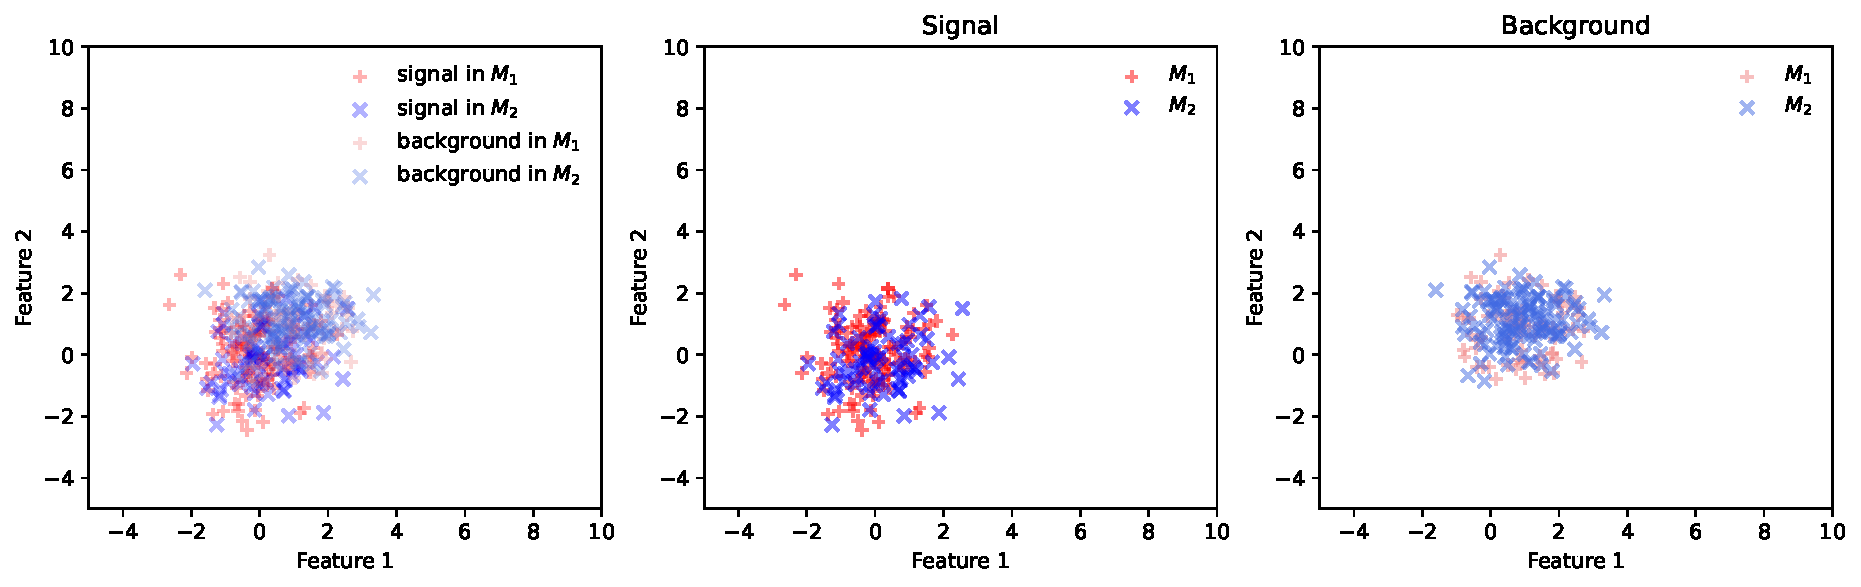
\includegraphics[width=0.97\textwidth]{bootstrapping_training_data_original.pdf}
        \caption{The signal and background samples distributions. The signal and background events are sampled from different two-dimensional normal distributions. They are randomly assigned to the mixed datasets $M_1$ or $M_2$.}
        \label{fig:bootstrapping_signal_background_distribution_origin}
    \end{figure}
    \begin{figure}[htpb]
        \centering
        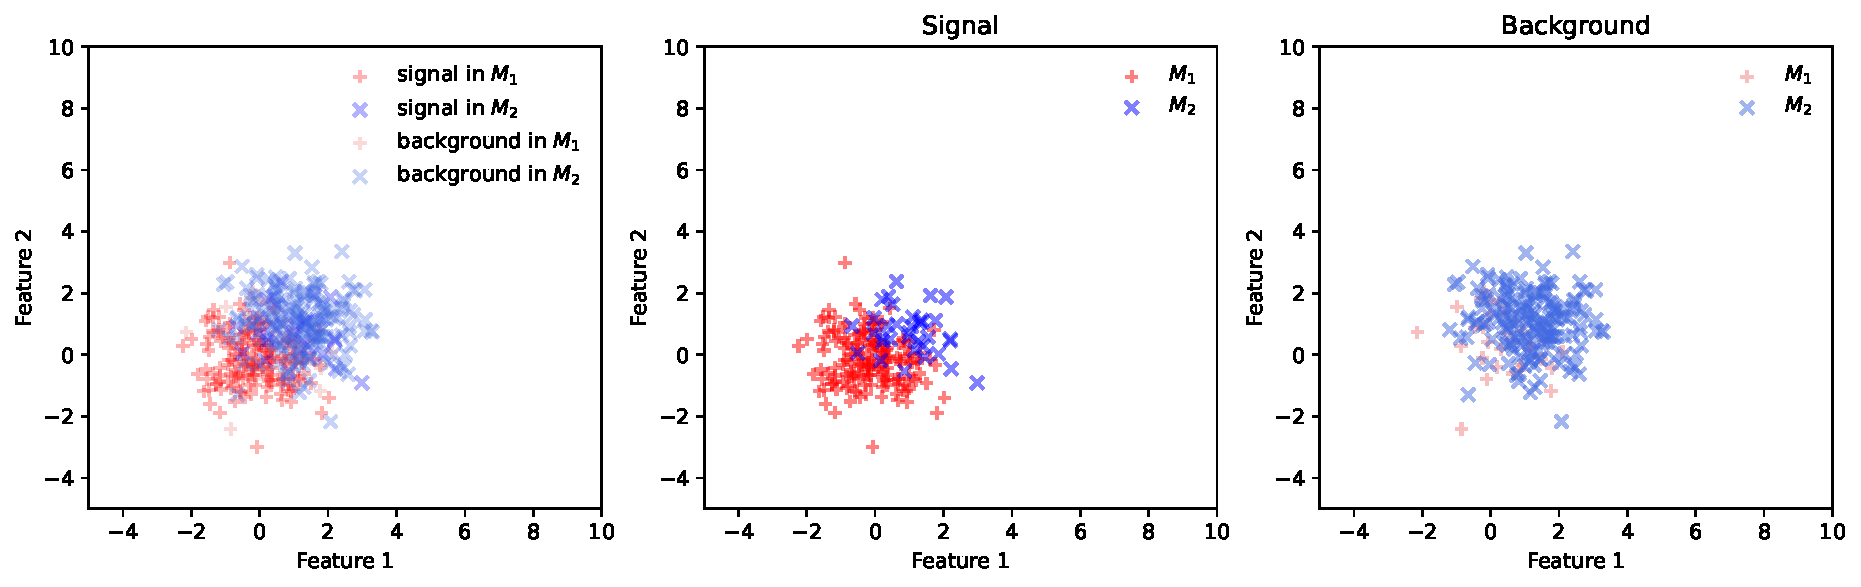
\includegraphics[width=0.97\textwidth]{bootstrapping_training_data_iteration_1.pdf}
        \caption{The signal and background samples distributions. The signal and background events are sampled from different two-dimensional normal distributions. The trained classifier assigns them to the $M_1$ or $M_2$.}
        \label{fig:bootstrapping_signal_background_distribution_iteration_1}
    \end{figure}
% section bootstrapping (end)
\section{Multi-class CWoLa}% (fold)
\label{sec:multi_class_cwola}
    The original CWoLa is only applied to the binary classification tasks. We want to extend the traditional CWoLa to more than two classes.

    \subsection{Dataset and model setup}% (fold)
    \label{sub:dataset_and_model_setup}
        We consider three pure samples, denoted by $A, B$, and $C$. The mixed datasets are denoted by $M_1, M_2$, and $M_3$. The training dataset is sampled from 5-dimensional normal distributions. Each mixed dataset has 10,000 events. The testing dataset consists of 1,000 pure samples for each class.

        The neural network consists of two dense layers with eight hidden nodes. The loss function is categorical cross-entropy. To prevent over-training, we utilize the early stopping technique with patience 10. The output is a 3-dimensional vector, and each component can be interpreted as the probability belonging to each type.
    % subsection dataset_and_model_setup (end)
    \subsection{Dominated case}% (fold)
    \label{sub:dominated_case}
        To simplify the problem, we start by considering a case where each pure class dominates different mixed samples. This would help us understand the behavior of the multi-class classifier before going to more complex scenarios.

        Table~\ref{tab:type_fraction_dominated_1} lists the fractions of pure samples in mixed datasets. Each mixed dataset is dominated by one pure sample type. Figure~\ref{fig:pure_sample_distribution_dominated_1} illustrates the distributions of the pure classes within these datasets.
        \begin{table}[htpb]
            \centering
            \caption{Fractions of pure samples in mixed datasets.}
            \label{tab:type_fraction_dominated_1}
            \begin{tabular}{c|ccc}
                Dataset & $A$  & $B$  & $C$  \\ \hline
                $M_1$   & 0.70 & 0.20 & 0.10 \\
                $M_2$   & 0.10 & 0.70 & 0.20 \\
                $M_3$   & 0.20 & 0.10 & 0.70
            \end{tabular}
        \end{table}
        \begin{figure}[htpb]
            \centering
            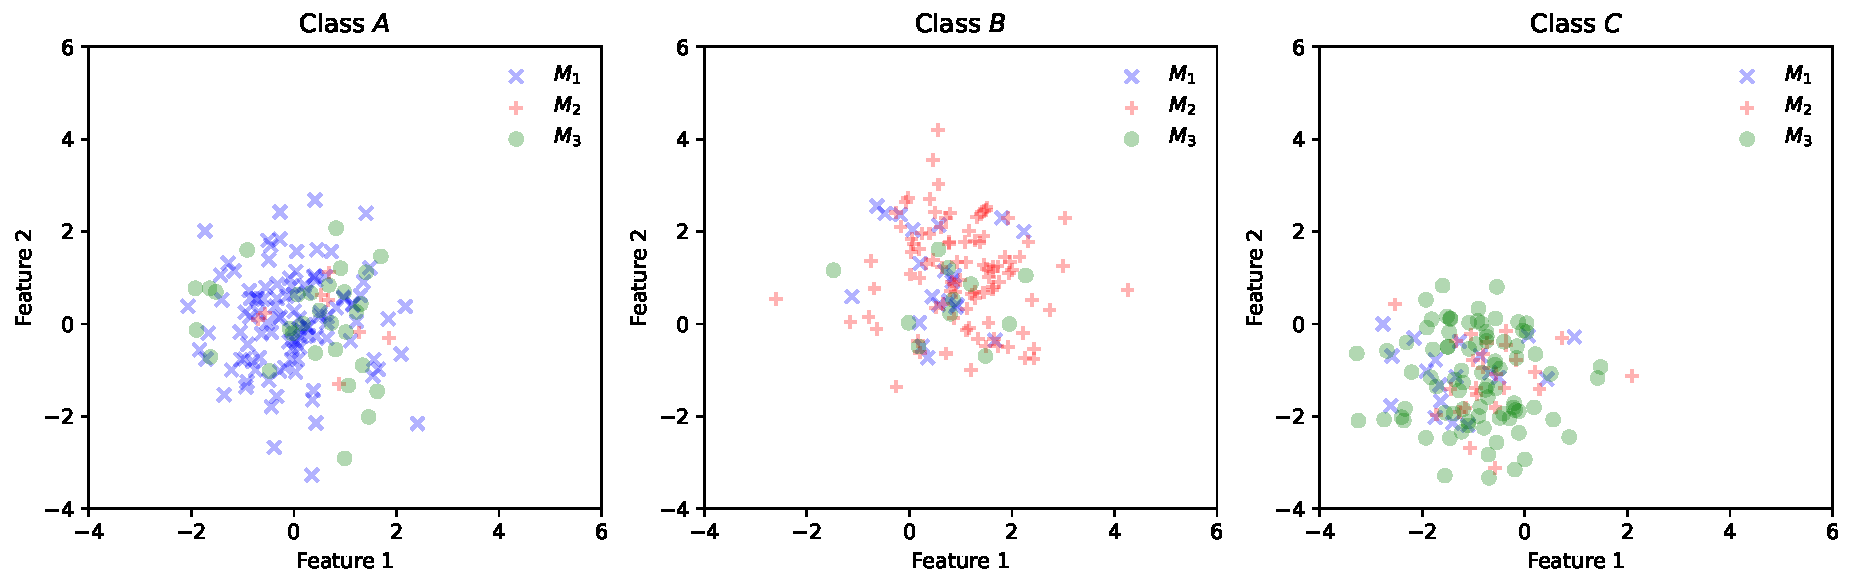
\includegraphics[width=0.97\textwidth]{multi-class_training_data-dominated_1.pdf}
            \caption{Distributions of pure samples in the mixed datasets. The classes $A, B$, and $C$ are sampled from the normal distribution with mean values $0, 1, -1$, respectively.}
            \label{fig:pure_sample_distribution_dominated_1}
        \end{figure}

        If the output vector suggests that the first type has the highest probability for dominated cases, it can be directly interpreted as belonging to the class $A$. The same logic applies to classes $B$ and $C$.  

        The event scores are the components of the output vector. Since the sum of event scores is always 1, we use the ternary plots to represent the event score distributions. In these plots, the coordinate of a point should be read following the direction of the ticks on each axis. 

        Figure~\ref{fig:event_score_distribution_dominated_1} shows the scatter plots of output vectors. The event score distributions are well-separated for each class, indicating successful training. The connections from regions 2 to 1 to 3, due to the mean value of class $B, A$, and $C$, are $1, 0$, and $-1$, respectively.  
        \begin{figure}[htpb]
            \centering
            \subfloat[Training data]{
                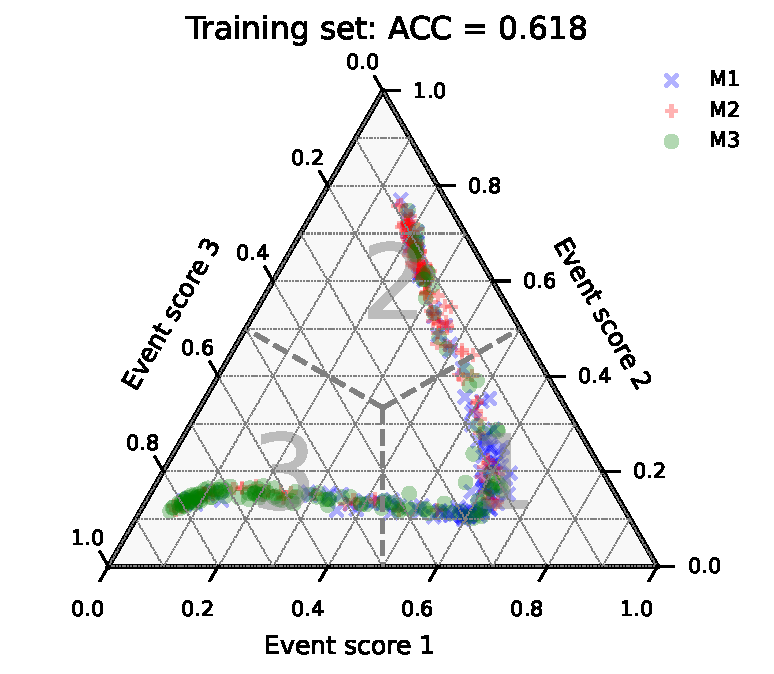
\includegraphics[width=0.47\textwidth]{multi-class_training_data_score-dominated_1.pdf}
            } 
            \subfloat[Testing data]{
                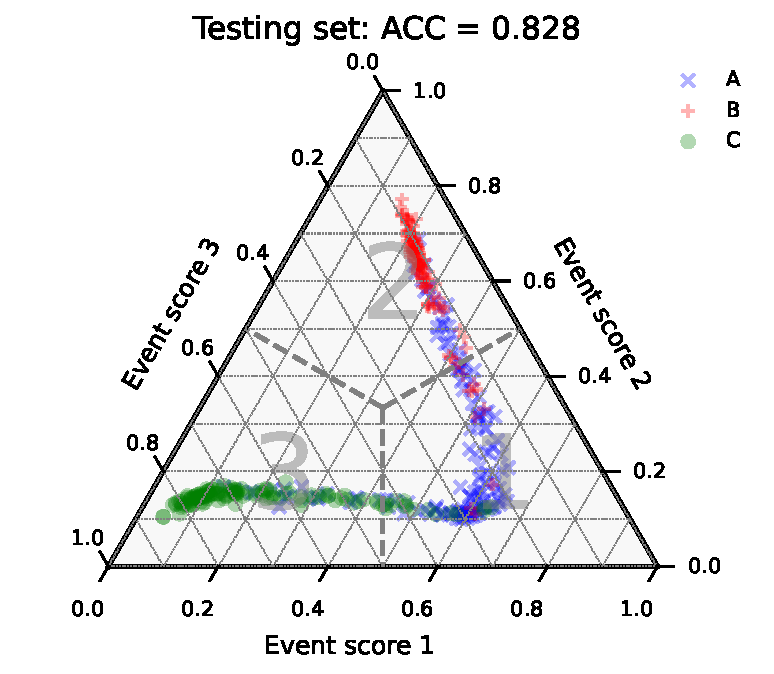
\includegraphics[width=0.47\textwidth]{multi-class_testing_data_score-dominated_1.pdf}
            } 
            \caption{Ternary plots of event score distributions. The grey dashed lines separate the regions corresponding to different classification results. The total accuracy (ACC) and the accuracy for each type are displayed.}
            \label{fig:event_score_distribution_dominated_1}
        \end{figure}  

        Table~\ref{tab:type_fraction_dominated_2} presents another type of the dominated case. Although the pure sample $A$ has the largest fraction in each mixed dataset, the pure class is still dominant in different mixed datasets. Figure~\ref{fig:pure_sample_distribution_dominated_2} illustrates the distributions of the pure classes in these datasets.  
        \begin{table}[htpb]
            \centering
            \caption{Fractions of pure samples in mixed datasets.}
            \label{tab:type_fraction_dominated_2}
            \begin{tabular}{c|ccc}
                Dataset & $A$  & $B$  & $C$  \\ \hline
                $M_1$   & 0.80 & 0.10 & 0.10 \\
                $M_2$   & 0.70 & 0.25 & 0.05 \\
                $M_3$   & 0.60 & 0.20 & 0.20
            \end{tabular}
        \end{table}  

        \begin{figure}[htpb]
            \centering
            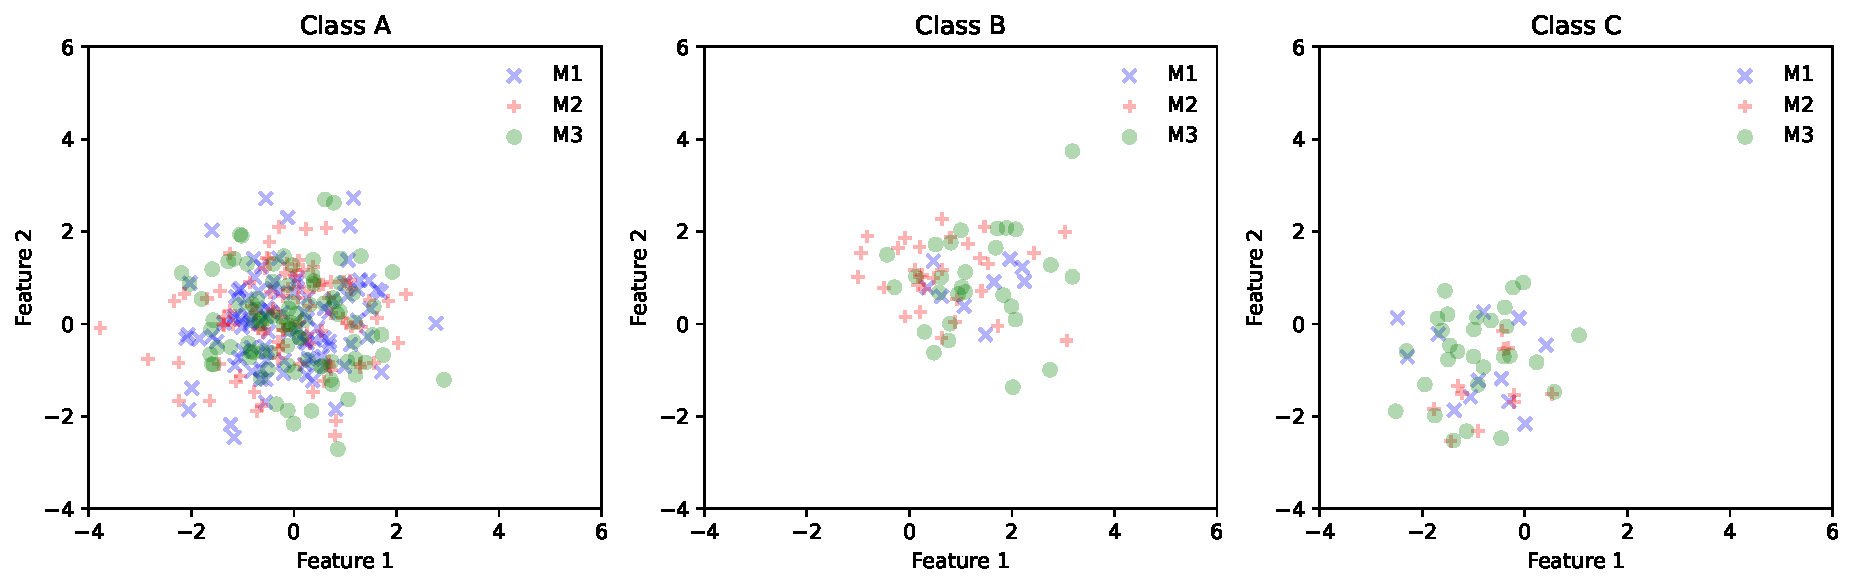
\includegraphics[width=0.97\textwidth]{multi-class_training_data-dominated_2.pdf}
            \caption{Distributions of pure samples in the mixed datasets. The classes $A$, $B$, and $C$ are sampled from normal distributions with mean values $0$, $1$, and $-1$, respectively.}
            \label{fig:pure_sample_distribution_dominated_2}
        \end{figure}  

        Figure~\ref{fig:event_score_distribution_dominated_2} shows scatter plots of output vectors. Although the training accuracy is not good, the testing results demonstrate excellent performance.
        \begin{figure}[htpb]
            \centering
            \subfloat[Training data]{
                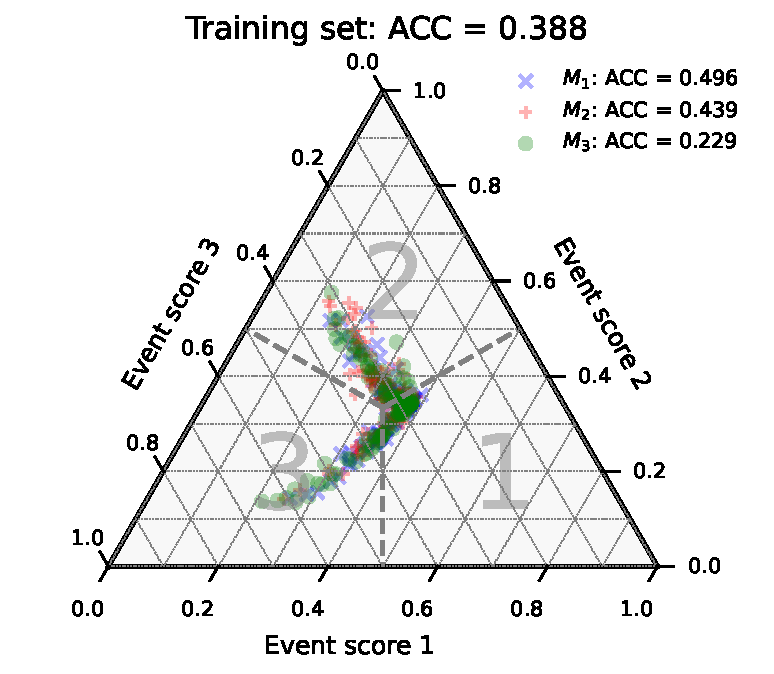
\includegraphics[width=0.47\textwidth]{multi-class_training_data_score-dominated_2.pdf}
            } 
            \subfloat[Testing data]{
                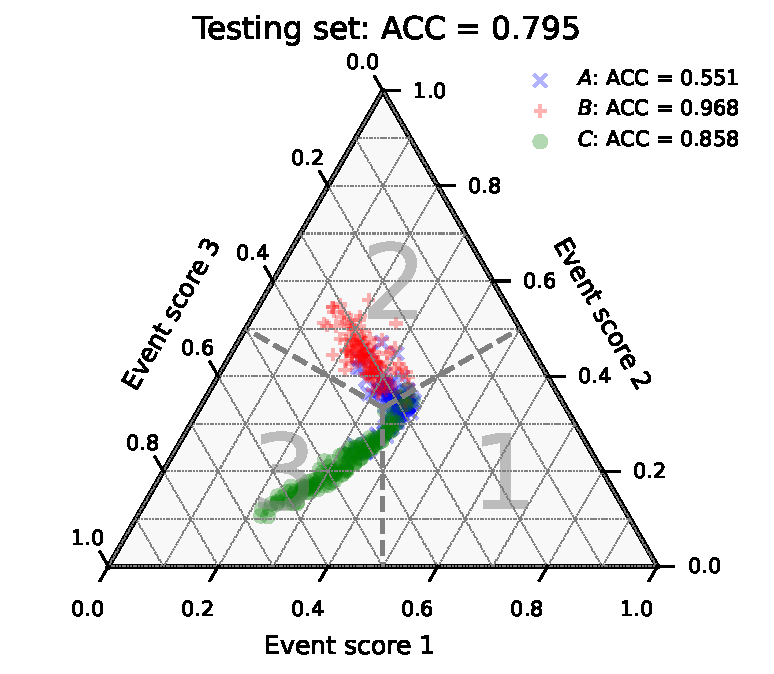
\includegraphics[width=0.47\textwidth]{multi-class_testing_data_score-dominated_2.pdf}
            } 
            \caption{Ternary plots of event score distributions. The grey dashed lines separate the regions corresponding to different classification results. The total accuracy (ACC) and the accuracy for each type are displayed.}
            \label{fig:event_score_distribution_dominated_2}
        \end{figure}

        From these results, we can conclude the ternary CWoLa works for dominated cases.
    % subsection dominated_case (end)
    \subsection{Ambiguous case}% (fold)
    \label{sub:ambiguous_case}
        Table~\ref{tab:type_fraction_ambiguous} lists the fractions of pure samples in mixed datasets. The ambiguous cases mean that the pure sample is not dominant in different mixed datasets. For instance, in table~\ref{tab:type_fraction_ambiguous}, pure samples $B$ and $C$ both dominate in $M_3$. Figure~\ref{fig:pure_sample_distribution_ambiguous} illustrates the distributions of the pure classes within these datasets.
        \begin{table}[htpb]
            \centering
            \caption{Fractions of pure samples in mixed datasets.}
            \label{tab:type_fraction_ambiguous}
            \begin{tabular}{c|ccc}
                Dataset & $A$  & $B$  & $C$  \\ \hline
                $M_1$   & 0.80 & 0.10 & 0.10 \\
                $M_2$   & 0.70 & 0.20 & 0.10 \\
                $M_3$   & 0.60 & 0.25 & 0.15
            \end{tabular}
        \end{table}
        \begin{figure}[htpb]
            \centering
            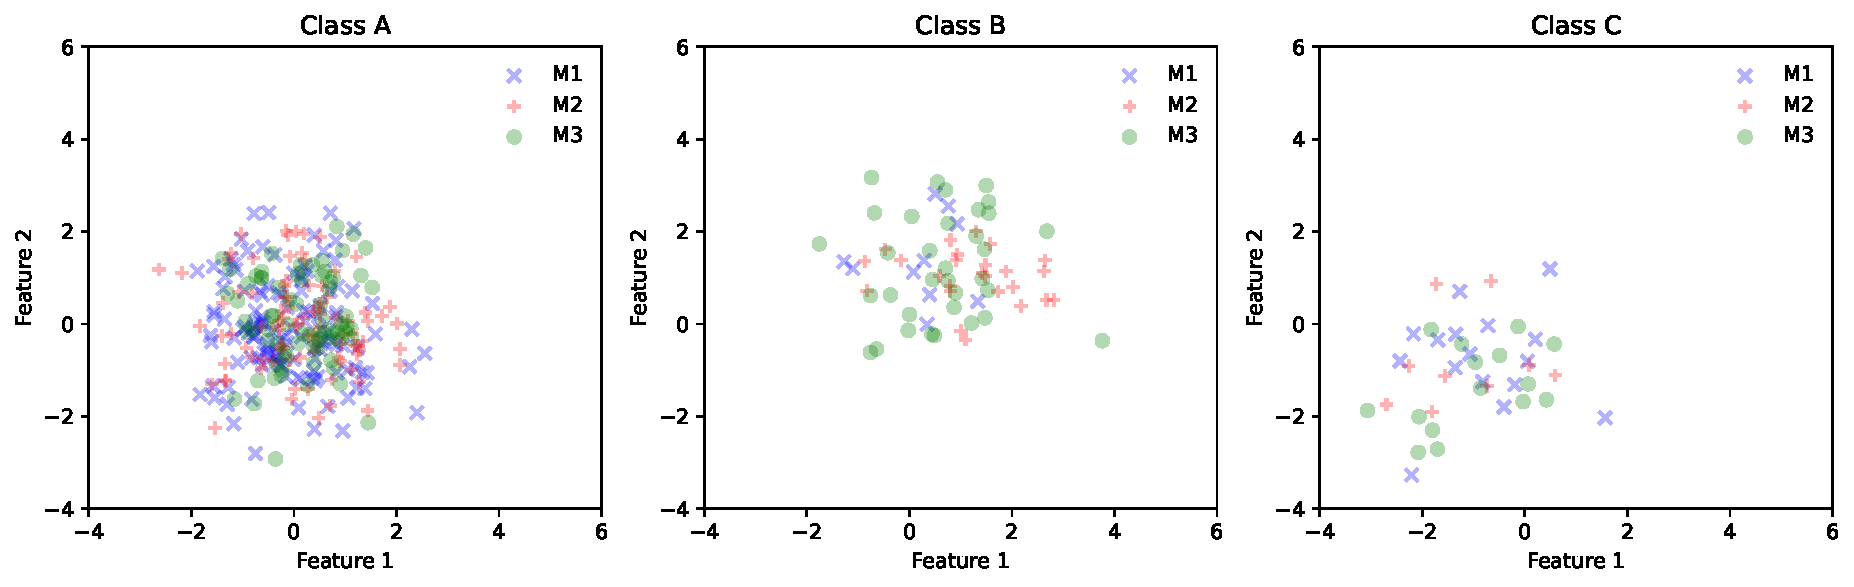
\includegraphics[width=0.97\textwidth]{multi-class_training_data-ambiguous.pdf}
            \caption{Distributions of pure samples in the mixed datasets. The classes $A, B$, and $C$ are sampled from the normal distribution with mean values $0, 1$, and $-1$, respectively.}
            \label{fig:pure_sample_distribution_ambiguous}
        \end{figure}

        For ambiguous cases, we apply the same logic to interpret the output vector as in dominated cases. However, the results could be problematic.

        Figure~\ref{fig:event_score_distribution_ambiguous} shows scatter plots of the output vectors. While the testing accuracy is very low, different types of pure samples exhibit distinct distributions. This suggests that we need another method to interpret the output vector. 

        Note that the accuracy for class $B$ is very low, while the accuracy for class $C$ is significantly higher. This suggests that when the classifier receives an event from either class $B$ or $C$, it tends to assign a high event score of type 3. This behavior is consistent with the fact that the pure samples $B$ and $C$ both are dominated in $M_3$. We need to refine our classification method or better interpret the output vectors to improve performance.
        \begin{figure}[htpb]
            \centering
            \subfloat[Training data]{
                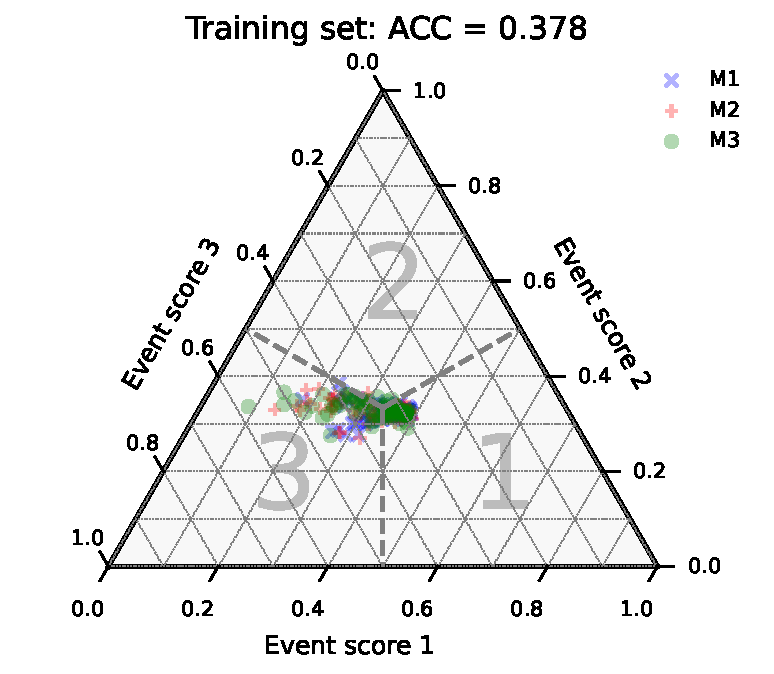
\includegraphics[width=0.47\textwidth]{multi-class_training_data_score-ambiguous.pdf}
            } 
            \subfloat[Testing data]{
                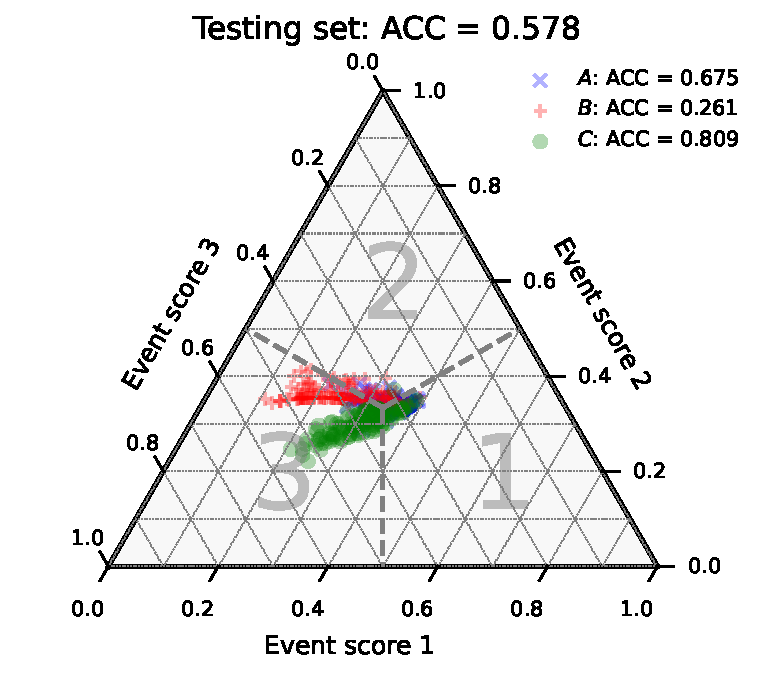
\includegraphics[width=0.47\textwidth]{multi-class_testing_data_score-ambiguous.pdf}
            } 
            \caption{Ternary plots of event score distributions. The grey dashed lines separate the regions corresponding to different classification results. The total accuracy (ACC) and the accuracy for each type are displayed.}
            \label{fig:event_score_distribution_ambiguous}
        \end{figure} 
    % subsection ambiguous_case (end)
% section multi_class_cwola (end)
\section{Output vector interpretation}% (fold)
\label{sec:output_vector_interpretation}
    In section~\ref{sec:multi_class_cwola}, the predicted label is determined from the output vector using the following method: if the first class has the highest probability, the sample is assigned to class $A$. The same logic applies to classes $B$ and $C$. We refer to this approach as the ``max argument'' method. 

    While this interpretation works well for dominant cases, it performs poorly for ambiguous cases. However, for such cases, the output vector distributions still differ between pure classes, suggesting that we need a better prediction method. The clustering algorithms might provide an alternative way to determine the type of a given sample.

    \subsection{Ambiguous case}% (fold)
    \label{sub:ambiguous_case}
        We consider the ambiguous cases described in section~\ref{sub:ambiguous_case} and test different clustering methods as alternative prediction strategies.

        Figure~\ref{fig:event_score_distribution_w_prediction_ambiguous} presents the prediction results for various methods, where colors represent the predicted labels. Both clustering approaches show improvements in overall accuracy. Table~\ref{tab:accuracy_w_different_prediction_ambiguous} summarizes the mean and standard deviation of accuracies for each prediction method. Notably, both clustering methods significantly improve the accuracy for pure class $B$, contributing to the observed increase in total accuracy.
       \begin{figure}[htpb]
            \centering
            \subfloat[Max argument method]{
                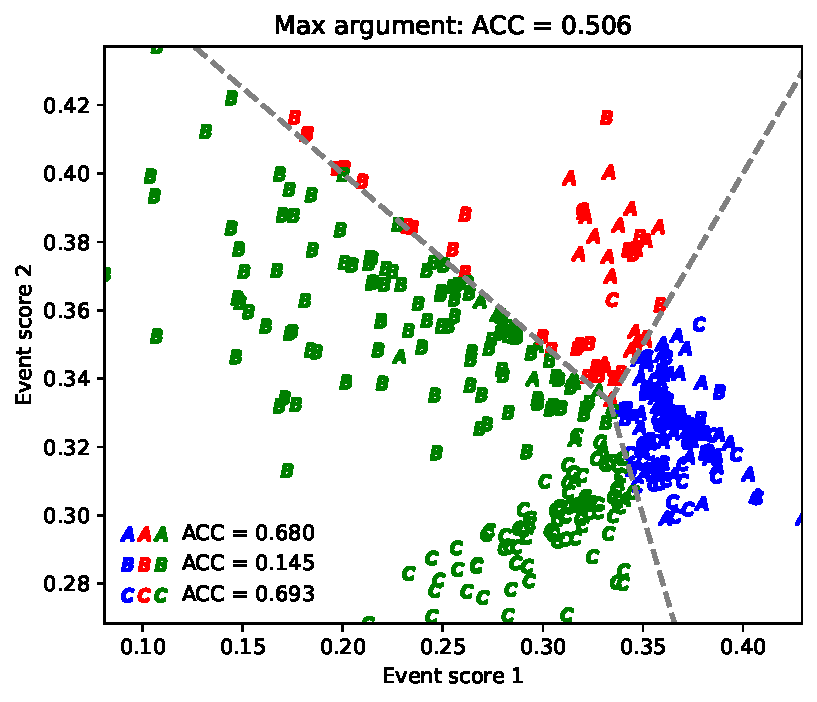
\includegraphics[width=0.47\textwidth]{multi-class_testing_data_predict-ambiguous-maxarg.pdf}
            } 
            \subfloat[K-means clustering]{
                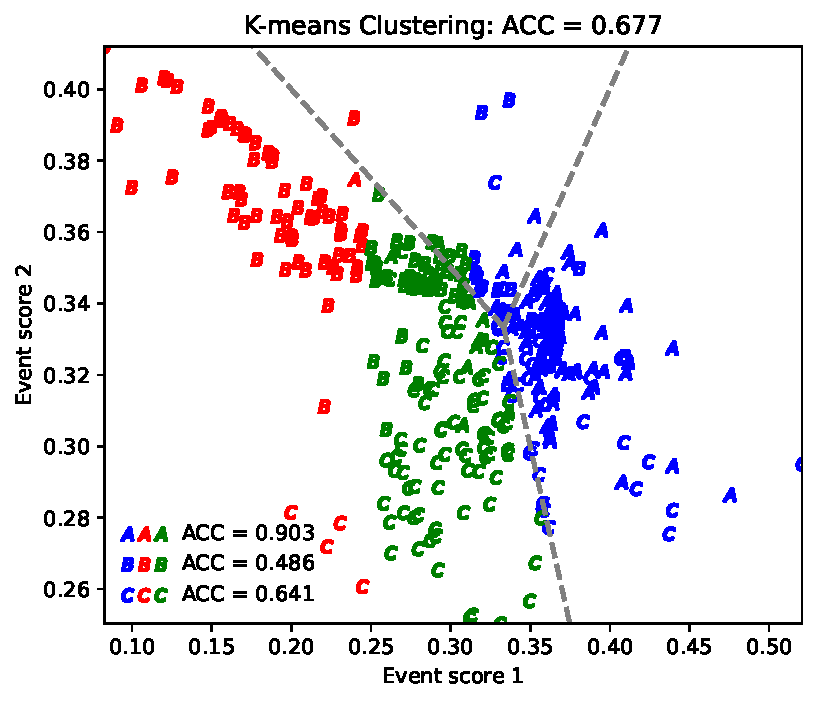
\includegraphics[width=0.47\textwidth]{multi-class_testing_data_predict-ambiguous-kmeans.pdf}
            } \\
            \subfloat[Spectral clustering]{
                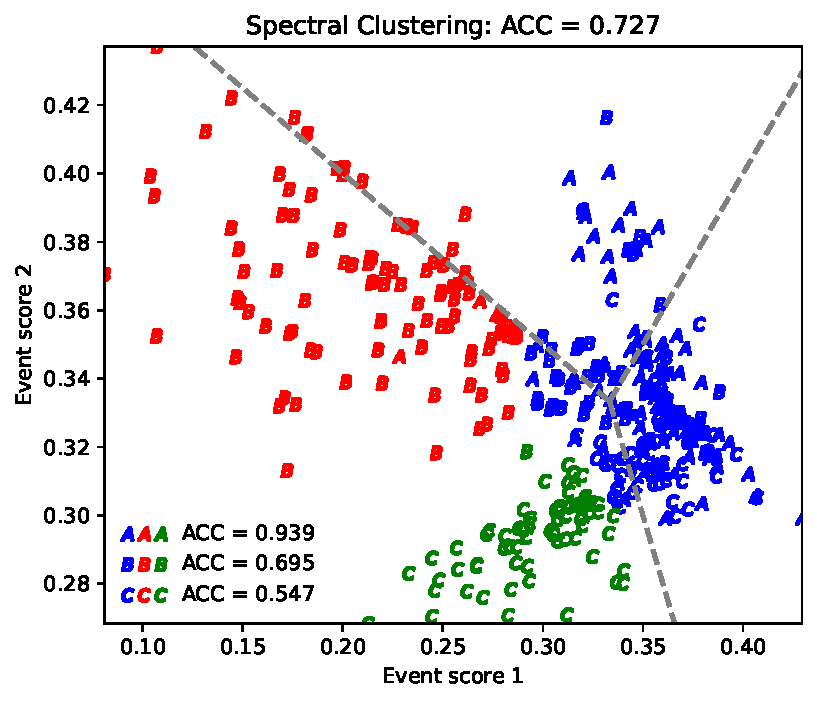
\includegraphics[width=0.47\textwidth]{multi-class_testing_data_predict-ambiguous-spectral.pdf}
            } 
            \caption{Event score distribution with prediction results. The grey dashed lines indicate regions corresponding to different predicted labels using the max argument method. The total accuracy and per-class accuracies are displayed.}
            \label{fig:event_score_distribution_w_prediction_ambiguous}
        \end{figure}
        \begin{table}[htpb]
            \centering
            \caption{Accuracy of different prediction methods. The means and standard deviations are computed over ten training runs.}
            \label{tab:accuracy_w_different_prediction_ambiguous}
            \begin{tabular}{c|ccc|c}
                Prediction Method   & $A$               & $B$               & $C$               & Total             \\ \hline
                Max argument        & $0.742 \pm 0.035$ & $0.164 \pm 0.100$ & $0.707 \pm 0.091$ & $0.538 \pm 0.027$ \\
                K-means clustering  & $0.868 \pm 0.028$ & $0.534 \pm 0.077$ & $0.595 \pm 0.050$ & $0.666 \pm 0.041$ \\
                Spectral clustering & $0.823 \pm 0.114$ & $0.625 \pm 0.096$ & $0.656 \pm 0.173$ & $0.702 \pm 0.061$
            \end{tabular}
        \end{table}
    % subsection ambiguous_case (end)
    \subsection{Dominant Case}  
    \label{sub:dominated_case}  
        We consider the dominant case described in table~\ref{tab:type_fraction_dominated_1} using different clustering methods as alternative prediction strategies.  

        Figure~\ref{fig:event_score_distribution_w_prediction_dominated_1} shows the prediction results for various methods. The three prediction methods exhibit similar performance. Since the max argument method already performs well, there is limited room for improvement.  

        Table~\ref{tab:accuracy_w_different_prediction_dominated_1} summarizes the mean and standard deviation of accuracies. While spectral clustering achieves better accuracy for class $A$, it performs worse for class $B$, resulting in a total accuracy that is approximately 2\% lower compared to the other prediction methods.  

        \begin{figure}[htpb]
            \centering
            \subfloat[Max argument method]{  
                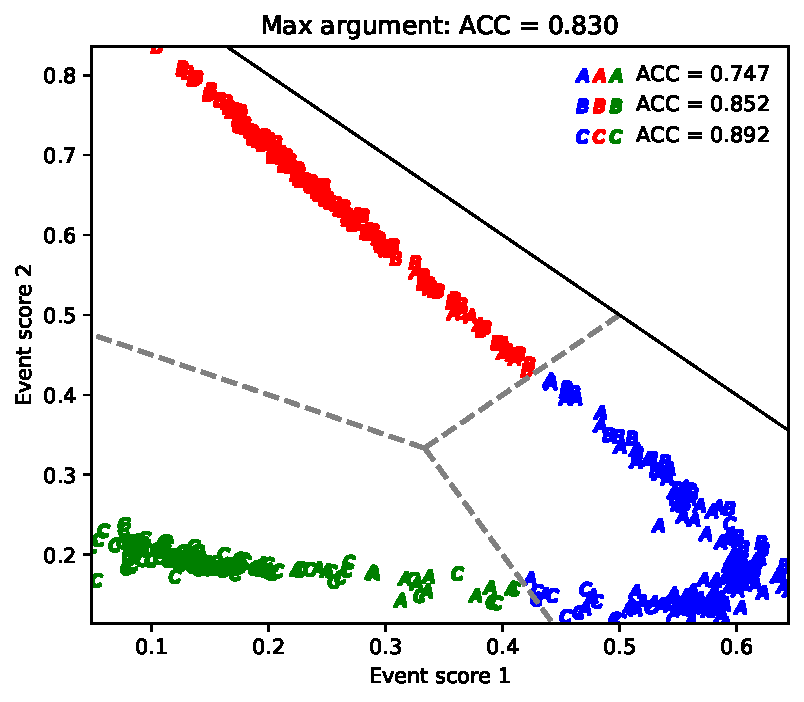
\includegraphics[width=0.47\textwidth]{multi-class_testing_data_predict-dominated_1-maxarg.pdf}  
            }  
            \subfloat[K-means clustering]{  
                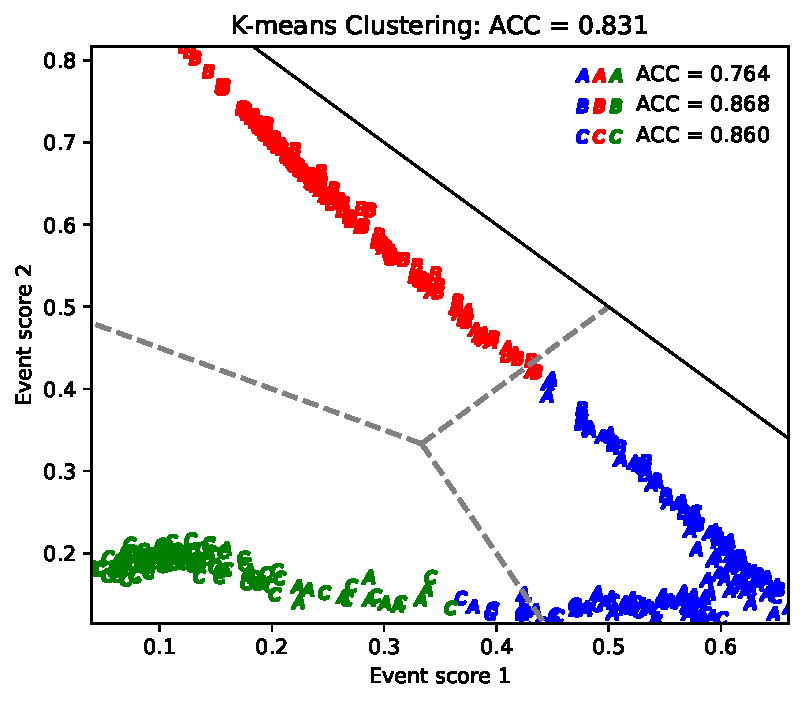
\includegraphics[width=0.47\textwidth]{multi-class_testing_data_predict-dominated_1-kmeans.pdf}  
            } \\  
            \subfloat[Spectral clustering]{  
                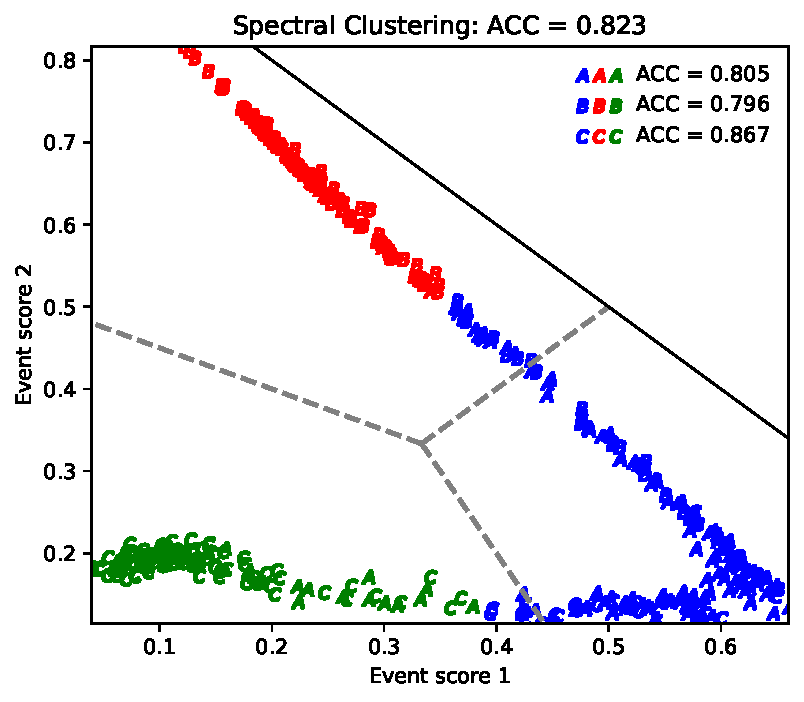
\includegraphics[width=0.47\textwidth]{multi-class_testing_data_predict-dominated_1-spectral.pdf}  
            }  
            \caption{Event score distribution with prediction results. The grey dashed lines indicate regions corresponding to different predicted labels using the max argument method. The black solid line represents the event score boundary. Total accuracy and per-class accuracies are displayed.}  
            \label{fig:event_score_distribution_w_prediction_dominated_1}  
        \end{figure}  

        \begin{table}[htpb]  
            \centering  
            \caption{Accuracy of different prediction methods. Means and standard deviations are computed over ten training runs.}  
            \label{tab:accuracy_w_different_prediction_dominated_1}  
            \begin{tabular}{c|ccc|c}  
                Prediction Method   & $A$               & $B$               & $C$               & Total             \\ \hline  
                Max argument        & $0.755 \pm 0.040$ & $0.824 \pm 0.025$ & $0.884 \pm 0.021$ & $0.821 \pm 0.003$ \\  
                K-means clustering  & $0.784 \pm 0.020$ & $0.828 \pm 0.017$ & $0.857 \pm 0.017$ & $0.823 \pm 0.003$ \\  
                Spectral clustering & $0.813 \pm 0.029$ & $0.746 \pm 0.019$ & $0.864 \pm 0.019$ & $0.807 \pm 0.005$  
            \end{tabular}  
        \end{table}  
    % subsection dominated_case (end)
% section output_vector_interpretation (end)
\section{Differences between training and testing sets}% (fold)
\label{sec:differences_between_training_and_testing_sets}
    In real applications, we only have training datasets and cannot obtain the true labels of the samples. Therefore, it is crucial to ensure that the performance of the training and testing datasets is similar, allowing prediction workflows to be effectively applied back to the training sets.

    \subsection{Dominant Case}% (fold)
    \label{sub:dominated_case_train_test_comparison}
        For the dominant case described in table~\ref{tab:type_fraction_dominated_1}, we evaluate different clustering methods as alternative prediction strategies.  

        Figure~\ref{fig:event_score_distribution_w_prediction_dominated_1_train_test_comparison} presents the prediction results for both training and testing datasets. The performance is consistent across the two datasets, with similar results for all three prediction methods. These findings are also consistent with the results discussed in section~\ref{sub:dominated_case} and demonstrate that the clustering prediction strategy can be effectively applied to training datasets.
        \begin{figure}[htpb]
            \centering
            \subfloat[Training sets]{  
                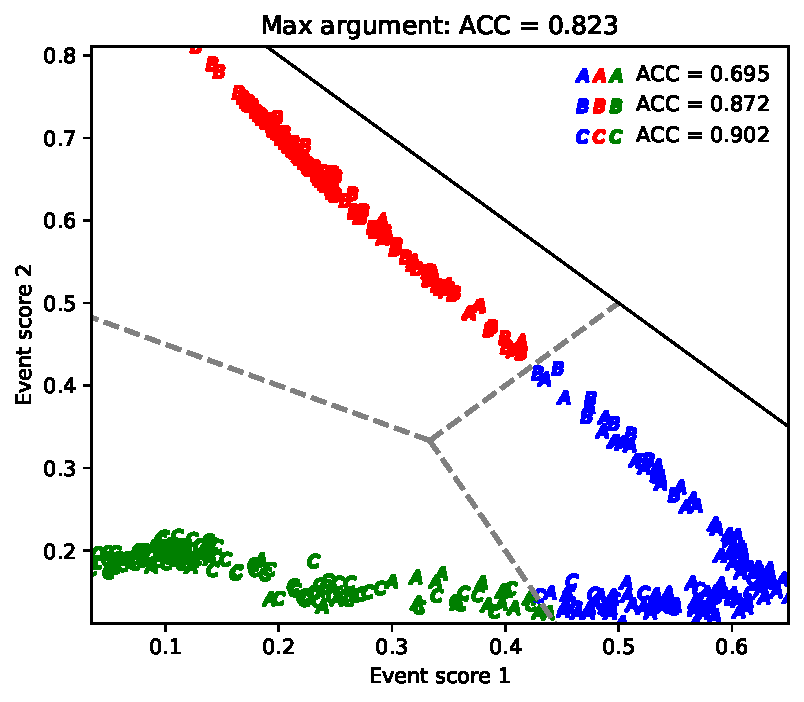
\includegraphics[width=0.38\textwidth]{multi-class_training_data_predict-dominated_1-maxarg.pdf}  
            }  
            \subfloat[Testing sets]{  
                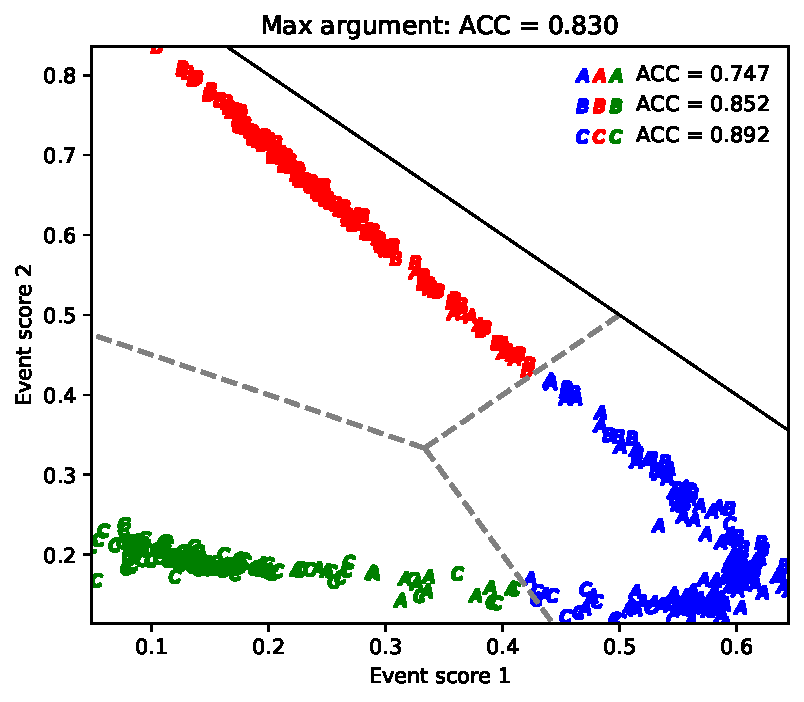
\includegraphics[width=0.38\textwidth]{multi-class_testing_data_predict-dominated_1-maxarg.pdf}  
            } \\  
            \subfloat[Training sets]{  
                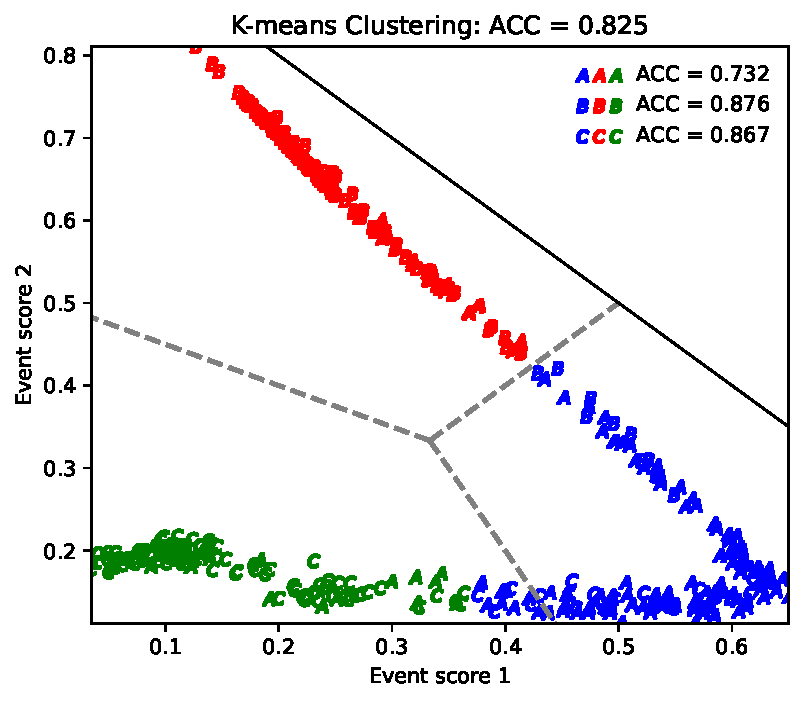
\includegraphics[width=0.38\textwidth]{multi-class_training_data_predict-dominated_1-kmeans.pdf}  
            }  
            \subfloat[Testing sets]{  
                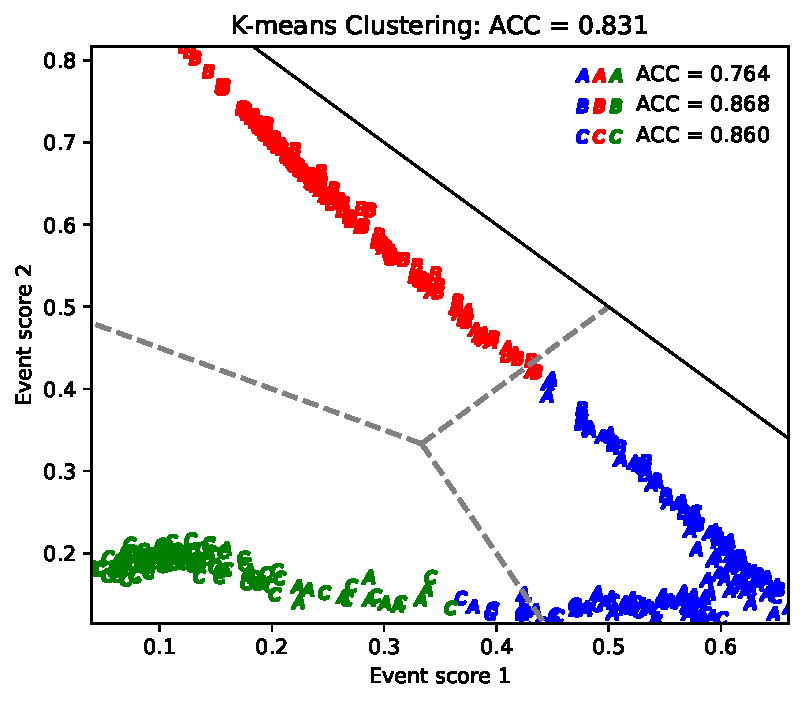
\includegraphics[width=0.38\textwidth]{multi-class_testing_data_predict-dominated_1-kmeans.pdf}  
            } \\  
            \subfloat[Training sets]{  
                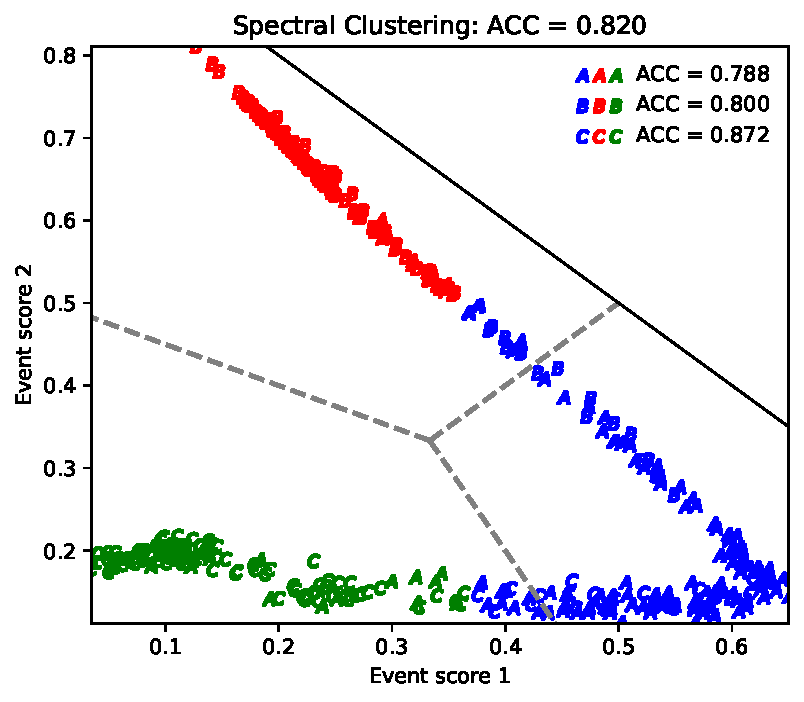
\includegraphics[width=0.38\textwidth]{multi-class_training_data_predict-dominated_1-spectral.pdf}  
            }  
            \subfloat[Testing sets]{  
                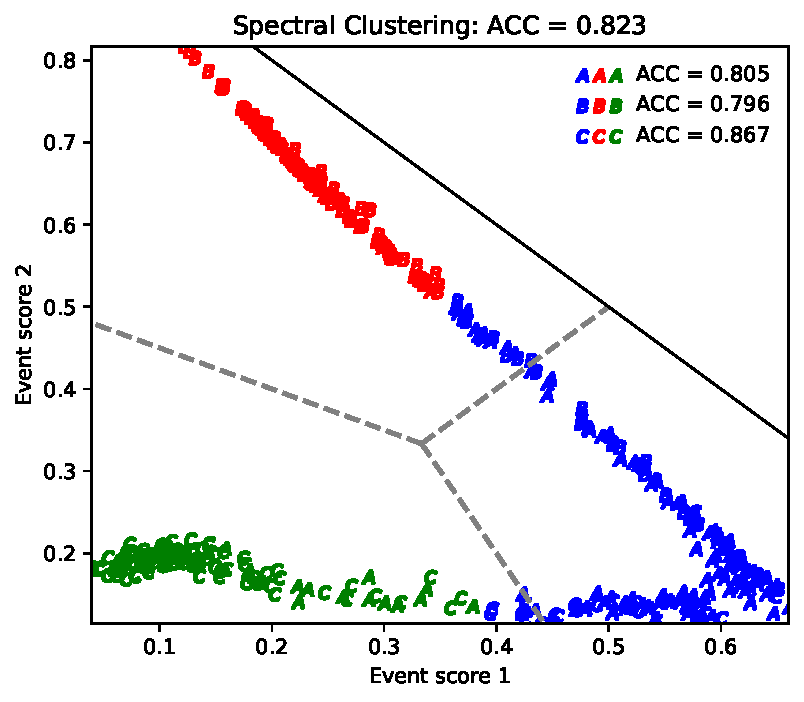
\includegraphics[width=0.38\textwidth]{multi-class_testing_data_predict-dominated_1-spectral.pdf}  
            }
            \caption{Event score distribution with prediction results. The grey dashed lines indicate regions corresponding to different predicted labels using the max argument method. The black solid line represents the event score boundary. Total accuracy and per-class accuracies are displayed.}  
            \label{fig:event_score_distribution_w_prediction_dominated_1_train_test_comparison}  
        \end{figure}  
    % subsection dominated_case_train_test_comparison (end)
    \subsection{Ambiguous Case}% (fold)
    \label{sub:ambiguous_case_train_test_comparison}
        We consider the ambiguous case described in table~\ref{tab:type_fraction_ambiguous} using different clustering methods as alternative prediction strategies.  

        Figure~\ref{fig:event_score_distribution_w_prediction_ambiguous_train_test_comparison} compares the prediction results for training and testing datasets. The training sets exhibit better performance for the Max-argument and K-means methods, whereas spectral clustering performs worse. The performance depends on the prediction method used.  

        Since the classifiers have been exposed to the training datasets, the training sample distribution should be more well-separated compared with the testing set. This could be the reason why the Max-argument and K-means methods have greater ACC on the training set. However, the poorer performance of spectral clustering on training sets is less clear, and we should explore it.
        \begin{figure}[htpb]
            \centering
            \subfloat[Training sets]{  
                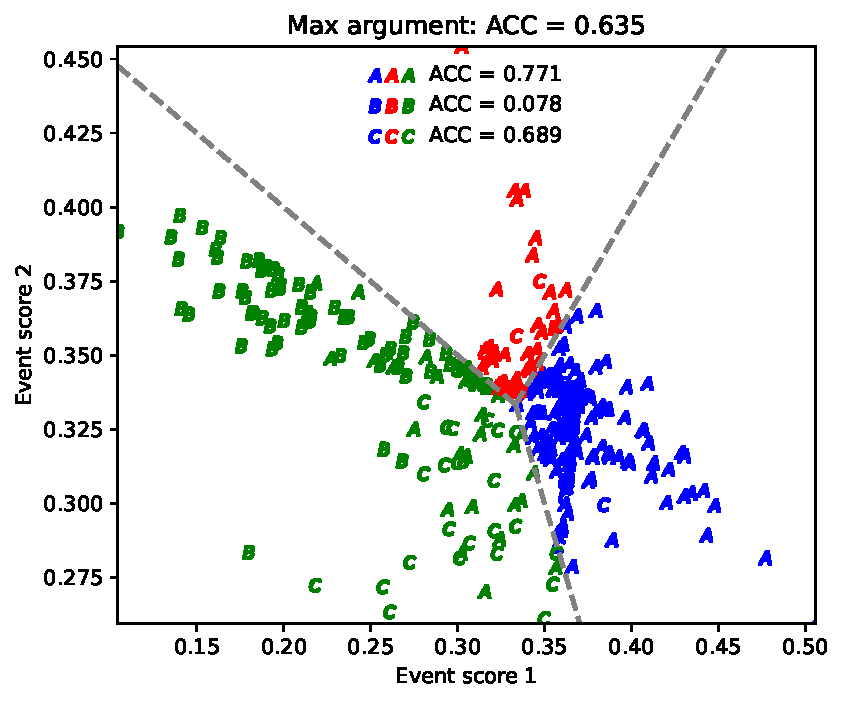
\includegraphics[width=0.39\textwidth]{multi-class_training_data_predict-ambiguous-maxarg.pdf}  
            }  
            \subfloat[Testing sets]{  
                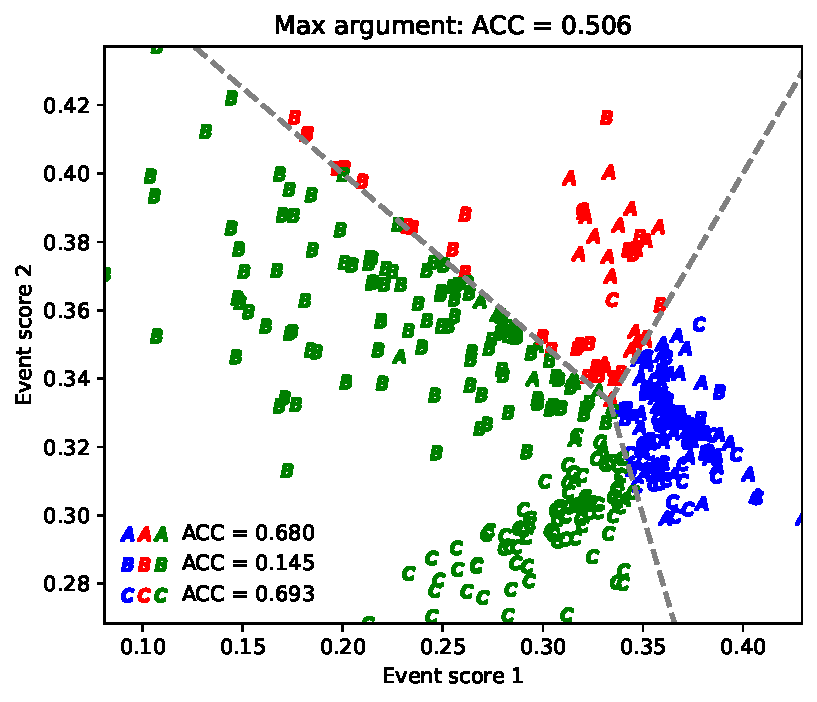
\includegraphics[width=0.39\textwidth]{multi-class_testing_data_predict-ambiguous-maxarg.pdf}  
            } \\  
            \subfloat[Training sets]{  
                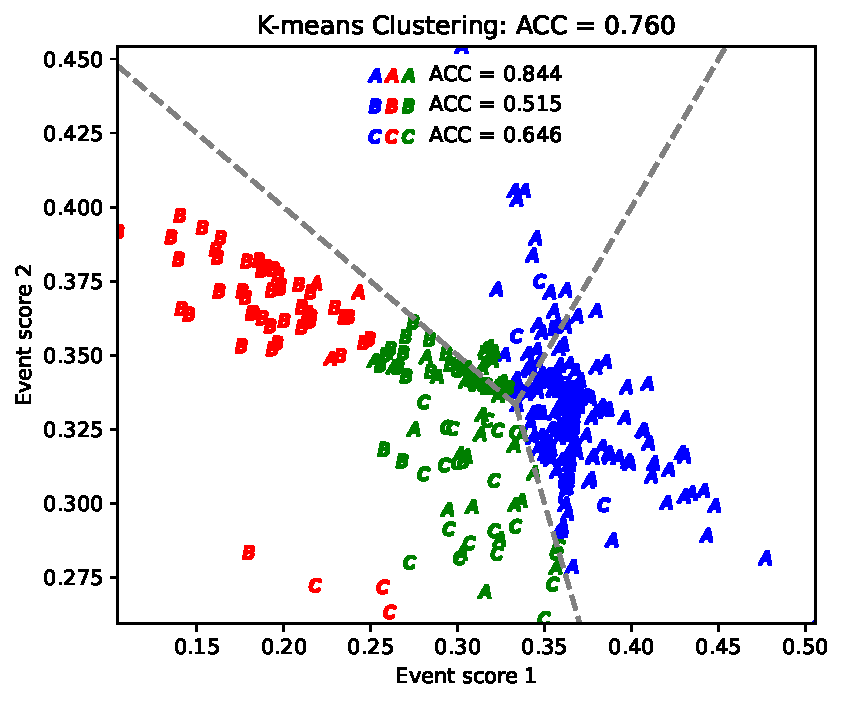
\includegraphics[width=0.39\textwidth]{multi-class_training_data_predict-ambiguous-kmeans.pdf}  
            }  
            \subfloat[Testing sets]{  
                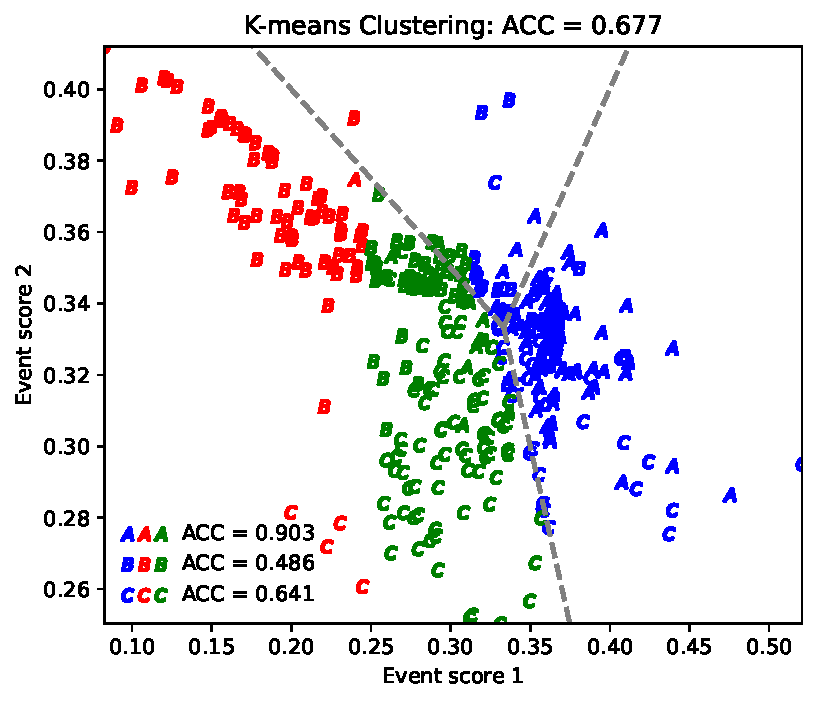
\includegraphics[width=0.39\textwidth]{multi-class_testing_data_predict-ambiguous-kmeans.pdf}  
            } \\  
            \subfloat[Training sets]{  
                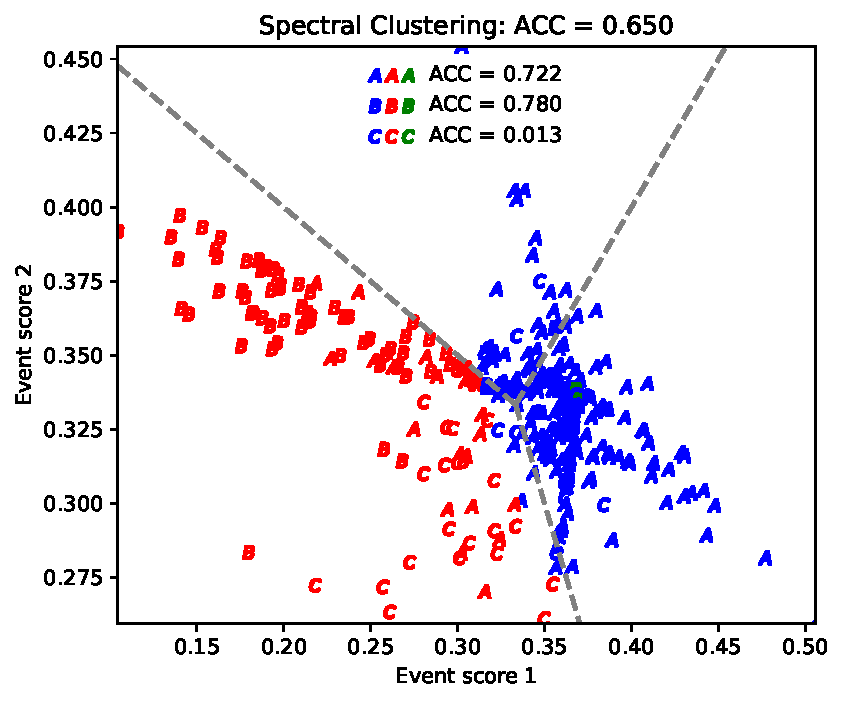
\includegraphics[width=0.39\textwidth]{multi-class_training_data_predict-ambiguous-spectral.pdf}  
            }  
            \subfloat[Testing sets]{  
                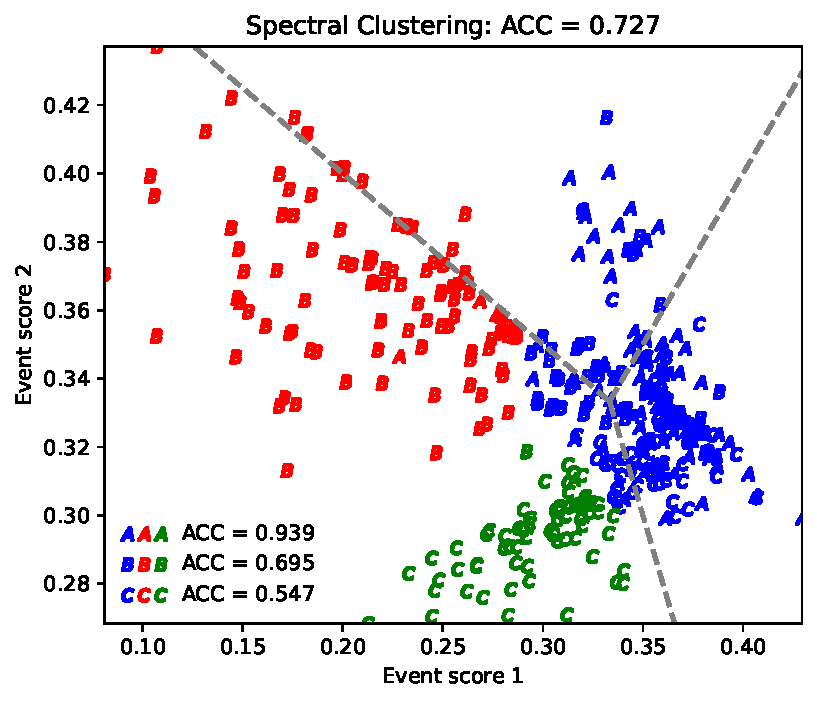
\includegraphics[width=0.39\textwidth]{multi-class_testing_data_predict-ambiguous-spectral.pdf}  
            }
            \caption{Event score distribution with prediction results. The grey dashed lines indicate regions corresponding to different predicted labels using the max argument method. The black solid line represents the event score boundary. Total accuracy and per-class accuracies are displayed.}  
            \label{fig:event_score_distribution_w_prediction_ambiguous_train_test_comparison}  
        \end{figure}
    % subsection ambiguous_case_train_test_comparison (end)
% section differences_between_training_and_testing_sets (end)
\section{Prediction Dependency Issue}  
\label{sec:prediction_dependency_issue}  

	When using clustering methods as alternative prediction strategies, the prediction results depend on the entire dataset, as the clustering process requires all samples to make predictions. To predict an event, we need to access the entire dataset.

	To address this prediction dependency issue, we propose training an additional neural network using the sample labels obtained from clustering-based predictions. This new neural network combines the functionalities of the CWoLa classifier (assigning event scores) and clustering-based prediction (final classification).

	The workflow consists of three steps:  
	\begin{enumerate}
		\item Train the initial neural network following the setup described in section~\ref{sub:dataset_and_model_setup}.  
		\item Apply a clustering prediction method to the training dataset to generate new labels.  
		\item Train a second neural network using the relabeled training dataset.  
	\end{enumerate}
	This second neural network should reproduce the performance of the original neural network combined with clustering-based prediction.  

	Table~\ref{tab:accuracy_w_different_prediction_dominated_1_combined_nn} summarizes the results for various prediction methods. ``K-means NN'' refers to the second neural network trained on K-means clustering labels. The results demonstrate that this approach performs similarly to directly applying clustering-based prediction on the original neural network. This finding suggests that a secondary neural network can effectively integrate the functionalities of a neural network and clustering-based prediction, removing the dependency on the entire dataset for predictions.  
	\begin{table}[htpb]  
		\centering  
		\caption{Accuracy of different prediction methods evaluated on the testing dataset. Means and standard deviations are calculated over ten training runs.}  
		\label{tab:accuracy_w_different_prediction_dominated_1_combined_nn}  
		\begin{tabular}{l|ccc|c}  
			Prediction Method   & $A$               & $B$               & $C$               & Total             \\ \hline  
			Max argument        & $0.751 \pm 0.027$ & $0.831 \pm 0.022$ & $0.884 \pm 0.017$ & $0.822 \pm 0.003$ \\  
			K-means clustering  & $0.782 \pm 0.015$ & $0.830 \pm 0.016$ & $0.856 \pm 0.018$ & $0.823 \pm 0.003$ \\  
			K-means NN          & $0.781 \pm 0.014$ & $0.831 \pm 0.018$ & $0.856 \pm 0.020$ & $0.823 \pm 0.003$ \\  
			Spectral clustering & $0.811 \pm 0.029$ & $0.768 \pm 0.026$ & $0.850 \pm 0.045$ & $0.810 \pm 0.007$ \\  
			Spectral NN         & $0.804 \pm 0.027$ & $0.762 \pm 0.025$ & $0.863 \pm 0.027$ & $0.810 \pm 0.005$  
		\end{tabular}  
	\end{table}  
% section prediction_dependency_issue (end)
\section{Physics process}% (fold)
\label{sec:physics_process}
    \subsection{Monte Carlo sample generation}% (fold)
    \label{sub:monte_carlo_sample_generation}
        We consider the following physics processes:  
        \begin{enumerate}
            \item The $Z'$ model process:
                \[
                    p p \to Z' \to W^{+}W^{-} \to \ell^{+} \nu_{\ell} \ell^{-}\overline{\nu}_{\ell}
                \] 
            \item SM process, $W^{+}W^{-}$ production:
                \[
                    p p \to W^{+}W^{-} \to \ell^{+}\nu_{\ell} \ell^{-}\overline{\nu}_{\ell}
                \]
            \item SM process, $ZZ$ production:
                \[
                    p p \to Z Z \to \ell^{+}\ell^{-} \nu_{\ell} \overline{\nu}_{\ell}
                \] 
        \end{enumerate}
        They all have the same final state. Thus, distinguishing these three production processes could be a real application of multi-class CWoLa.

        We adopt the $Z'$ model from this \href{http://feynrules.irmp.ucl.ac.be/wiki/HAHM#no1}{page}~\cite{Curtin:2013fra, Curtin:2014cca}. 

        We use \verb|MadGraph 3.3.1|~\cite{Alwall:2014hca} to generate these processes at a center-of-mass energy of $\sqrt{s} = 13$ TeV. The parton showering and hadronization are simulated using \verb|Pythia 8.306|~\cite{Sjostrand:2014zea}. The detector simulation is conducted by \verb|Delphes 3.4.2|~\cite{deFavereau:2013fsa}. Jet reconstruction is performed using \verb|FastJet 3.3.2|~\cite{Cacciari:2011ma} with the anti-$k_t$ algorithm~\cite{Cacciari:2008gp} and a jet radius of $R = 0.5$. These jets are required to have transverse momentum $p_{\text{T}} > 20$ GeV. We keep all settings as their default values for now.

        The following \verb|MadGraph| scripts generate Monte Carlo samples for each process.

        \paragraph{$Z'$ production}
        \begin{lstlisting}
            import model HAHM_variableMW_v5_UFO
            generate p p > zp > w+ w-, (w+ > l+ vl), (w- > l- vl~)
            output ppZp
            launch ppZp

            shower=Pythia8
            detector=Delphes
            analysis=OFF
            madspin=OFF
            done

            set run_card nevents 10000
            set run_card ebeam1 6500.0
            set run_card ebeam2 6500.0

            done
        \end{lstlisting}
        \paragraph{$W^{+}W^{-}$ production}
        \begin{lstlisting}
            generate p p > w+ w-, (w+ > l+ vl), (w- > l- vl~)
            output ppWpWm
            launch ppWpWm

            shower=Pythia8
            detector=Delphes
            analysis=OFF
            madspin=OFF
            done

            set run_card nevents 10000
            set run_card ebeam1 6500.0
            set run_card ebeam2 6500.0

            done
        \end{lstlisting}
        \paragraph{$ZZ$ production}
        \begin{lstlisting}
            generate p p > z z, (z > l+ l-), (z > vl vl~)
            output ppZZ
            launch ppZZ

            shower=Pythia8
            detector=Delphes
            analysis=OFF
            madspin=OFF
            done

            set run_card nevents 10000
            set run_card ebeam1 6500.0
            set run_card ebeam2 6500.0

            done
        \end{lstlisting}
    % subsection monte_carlo_sample_generation (end)
    \subsection{Event selection}% (fold)
    \label{sub:event_selection}
        The selection cuts after the \verb|Delphes| simulation:
        \begin{itemize}
            \item $n_{l}$ cut: The number of leptons (electron + muon) should be at least 2.
        \end{itemize}

        % Table~\ref{tab:GGF_VBF_Higgs_cutflow_number} summarizes the cutflow number at different selection cuts.
        % \begin{table}[htpb]
        %     \centering
        %     \caption{Number of passing events and passing rates for GGF and VBF Higgs production at different selection cuts.}
        %     \label{tab:GGF_VBF_Higgs_cutflow_number}
        %     \begin{tabular}{l|rr|rr}
        %         Cut                    & GGF    & pass rate & VBF    & pass rate \\ \hline
        %         Total                  & 100000 & 1         & 100000 & 1         \\
        %         $n_{\gamma}$ cut       & 48286  & 0.48      & 53087  & 0.53      \\
        %         $n_j$ cut              & 9302   & 0.09      & 42860  & 0.43      \\
        %         $m_{\gamma\gamma}$ cut & 8864   & 0.09      & 40694  & 0.41     
        %     \end{tabular}
        % \end{table}
        
        Figure~\ref{fig:mll_distribution} shows the distributions of $m_{ll}$ (the invariant mass of the two leading leptons).
        \begin{figure}[htpb]
            \centering
            \subfloat[$m_{ll}$ distribution]{
                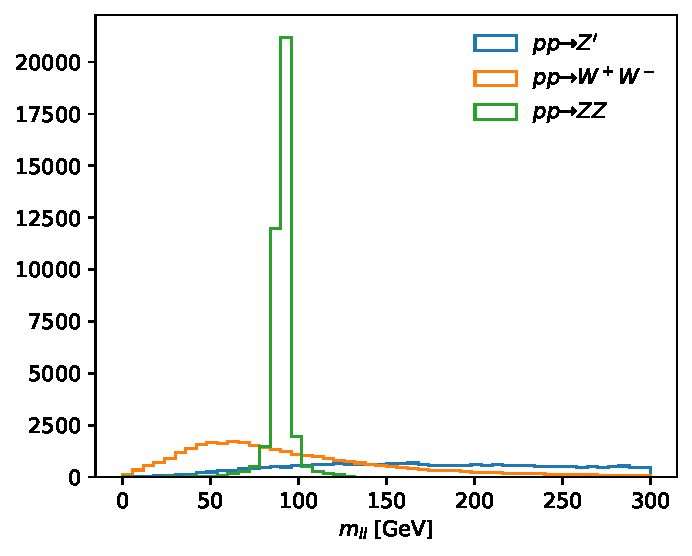
\includegraphics[width=0.60\textwidth]{mll_distribution.pdf}
            }
            \caption{Distributions of the invariant mass $m_{ll}$ of the two leading leptons.}
            \label{fig:mll_distribution}
        \end{figure}
    % subsection event_selection (end)
    \subsection{Event image}% (fold)
    \label{sub:event_image}
        The inputs for the neural networks are event images~\cite{Kasieczka:2019dbj,deOliveira:2015xxd, Kasieczka2017nv}. These images are constructed from events that pass the kinematic selection criteria described in section~\ref{sub:event_selection}. Each event image has three channels corresponding to calorimeter towers, track, and leptons. The following preprocessing steps are applied to all event constituents:
        \begin{enumerate}
            \item Translation: Compute the $p_{\text{T}}$-weighted center in the $\phi$ coordinates, then shift this point to the origin.
            \item Flipping: Flip the highest $p_{\text{T}}$ quadrant to the first quadrant.
            \item Pixelation: Pixelate in a $\eta \in [-5, 5],\ \phi \in [-\pi, \pi]$ box, with $40 \times 40$ pixels 
        \end{enumerate}

        Figure~\ref{fig:Zp_WW_ZZ_event_image} shows the event images for three different physics processes.
        \begin{figure}[htpb]
            \centering
            \subfloat[$Z'$: Calorimeter Tower]{
                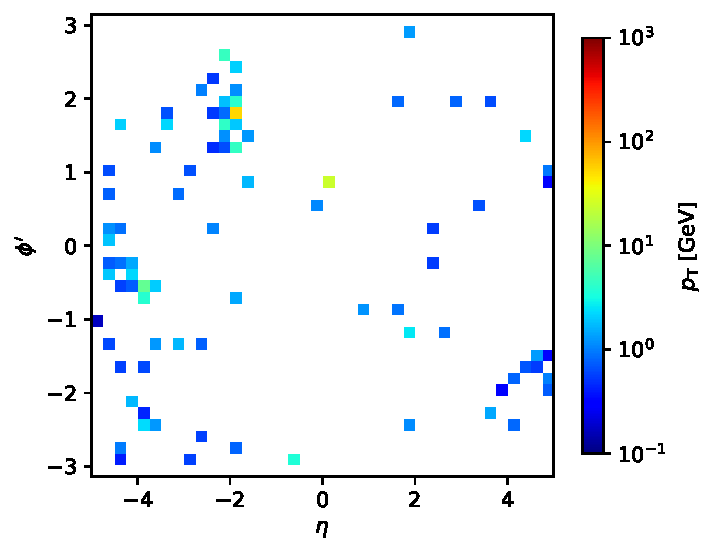
\includegraphics[width=0.31\textwidth]{event_image_ppZp-tower.pdf}
            }
            \subfloat[$W^+W^-$: Calorimeter Tower]{
                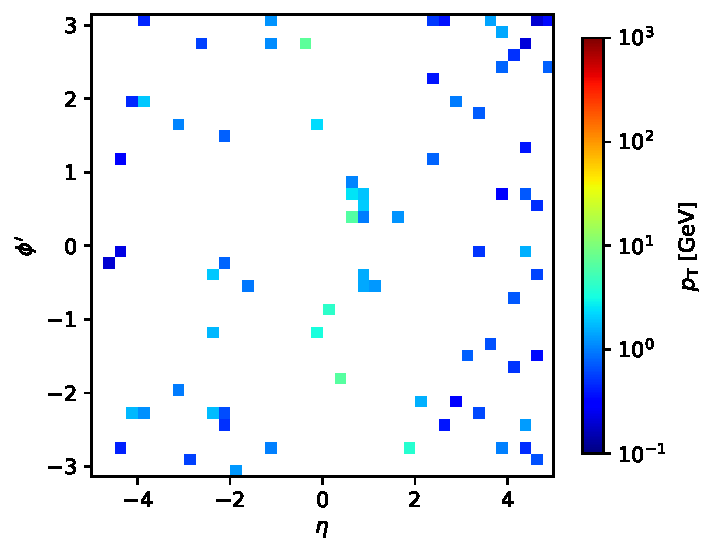
\includegraphics[width=0.31\textwidth]{event_image_ppWW-tower.pdf}
            }
            \subfloat[$ZZ$: Calorimeter Tower]{
                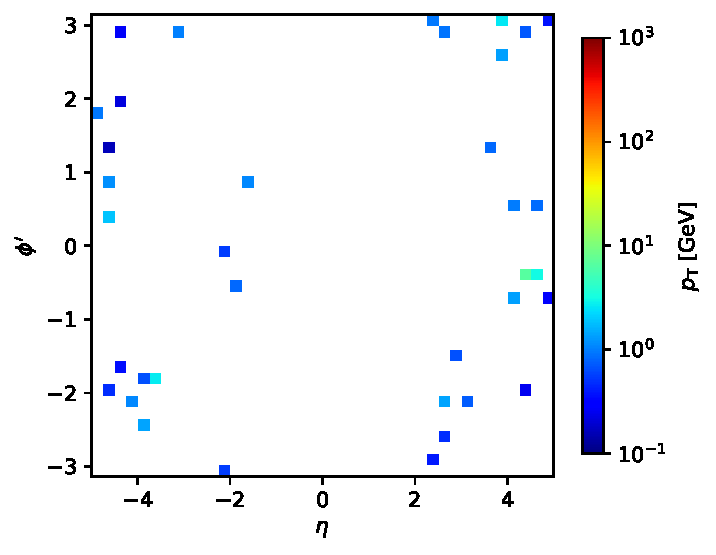
\includegraphics[width=0.31\textwidth]{event_image_ppZZ-tower.pdf}
            } \\
            \subfloat[$Z'$: Track]{
                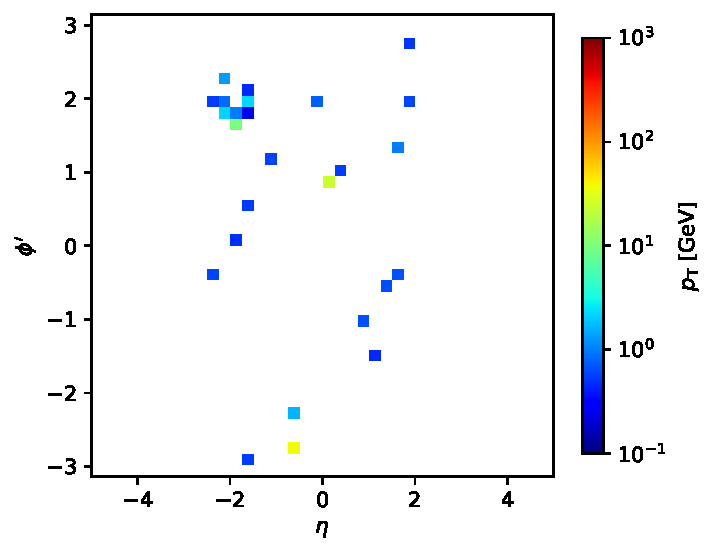
\includegraphics[width=0.31\textwidth]{event_image_ppZp-track.pdf}
            }
            \subfloat[$W^+W^-$: Track]{
                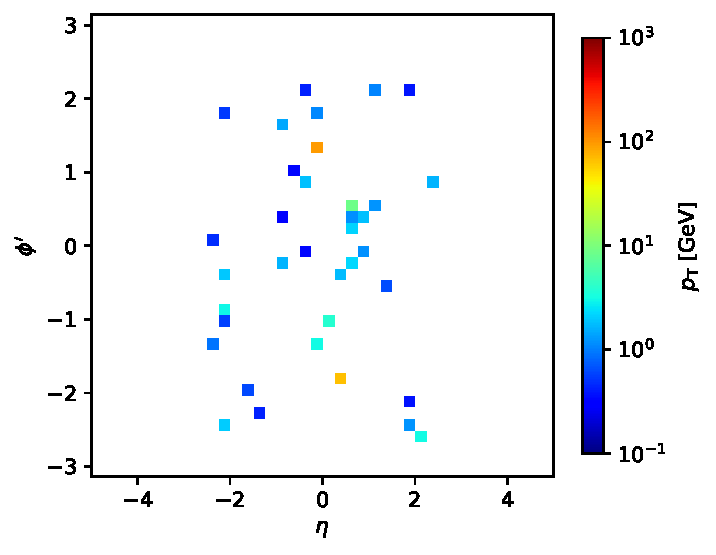
\includegraphics[width=0.31\textwidth]{event_image_ppWW-track.pdf}
            }
            \subfloat[$ZZ$: Track]{
                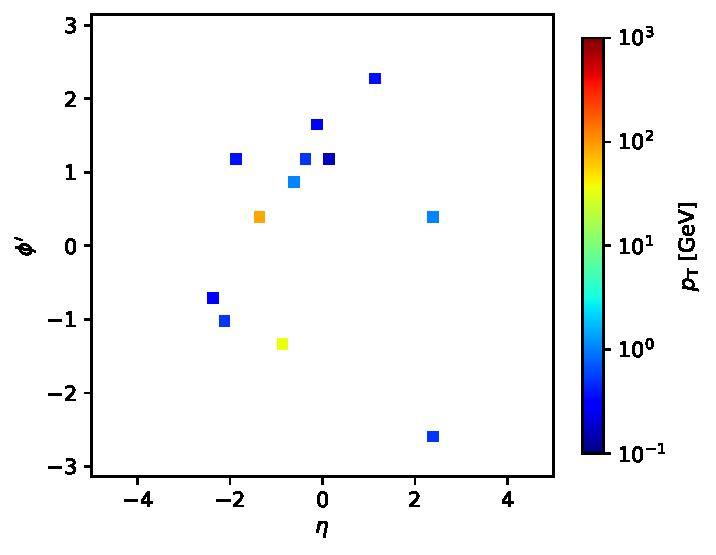
\includegraphics[width=0.31\textwidth]{event_image_ppZZ-track.pdf}
            } \\
            \subfloat[$Z'$: Lepton]{
                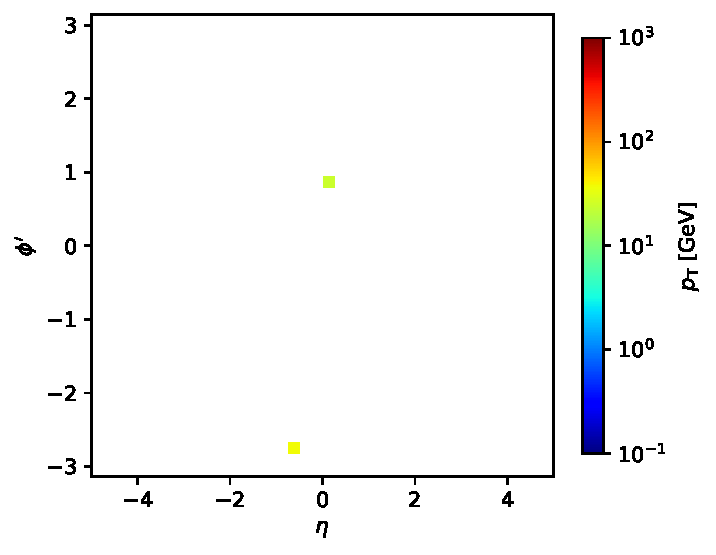
\includegraphics[width=0.31\textwidth]{event_image_ppZp-lepton.pdf}
            }
            \subfloat[$W^+W^-$: Lepton]{
                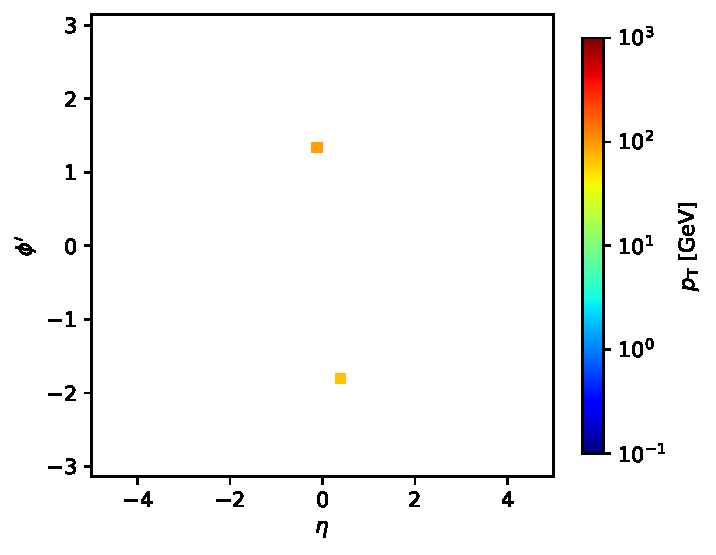
\includegraphics[width=0.31\textwidth]{event_image_ppWW-lepton.pdf}
            }
            \subfloat[$ZZ$: Lepton]{
                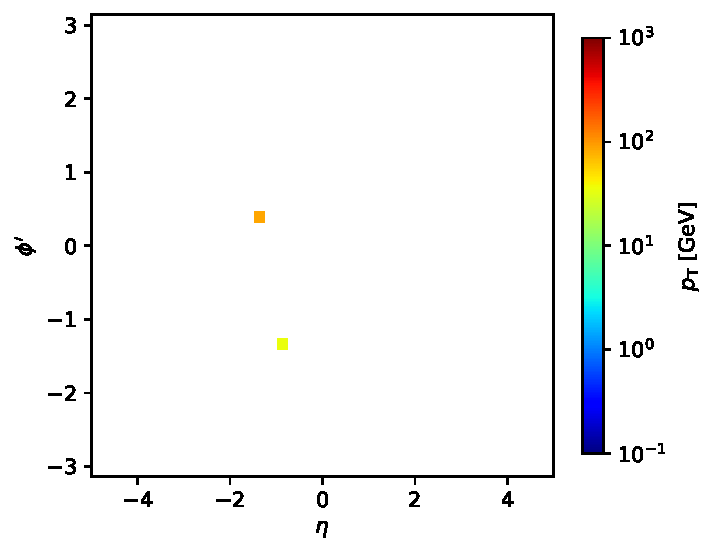
\includegraphics[width=0.31\textwidth]{event_image_ppZZ-lepton.pdf}
            }
            \caption{Event images for $Z', W^{+}W^{-}$, and $ZZ$ channel, separately shown for calorimeter towers, tracks, and leptons.}
            \label{fig:Zp_WW_ZZ_event_image}
        \end{figure}
    % subsection event_image (end)
% section physics_process (end)

\bibliographystyle{ieeetr}
\bibliography{reference}

\end{document}
